% =====================================================================
% UniBus Live — COMPLETE IEEE conference paper (single file)
% Compile on Overleaf (pdfLaTeX). IEEEtran is built into Overleaf.
%
% eta_accuracy_eval.sql; eyeball ref page-numbers on publisher pages.
% =====================================================================
\documentclass[conference]{IEEEtran}
\IEEEoverridecommandlockouts
\usepackage{cite}
\usepackage{amsmath,amssymb,amsfonts}
\usepackage{graphicx}
\usepackage{xcolor}
\usepackage{booktabs}
\usepackage{url}
\usepackage{tikz}
\usetikzlibrary{positioning, arrows.meta, calc, fit}
\usepackage{float}
\usepackage{algorithm}
\usepackage{algpseudocode}
\raggedbottom
\setlength{\intextsep}{4pt plus 1pt minus 1pt}
\setlength{\dbltextfloatsep}{11pt plus 2pt minus 3pt}
\def\BibTeX{{\rm B\kern-.05em{\sc i\kern-.025em b}\kern-.08em
  T\kern-.1667em\lower.7ex\hbox{E}\kern-.125emX}}

\definecolor{acc}{RGB}{28,60,102}
\newcommand{\stepnum}[1]{\tikz[baseline=-0.62ex]{\node[circle,fill=acc,text=white,
  inner sep=0.25mm, minimum size=3.1mm, font=\tiny\bfseries]{#1};}}
\tikzset{
  arr/.style={-{Latex[length=1.8mm,width=1.5mm]}, semithick, draw=black!80},
  barr/.style={-{Latex[length=1.8mm,width=1.5mm]}, semithick, draw=black!80, densely dashed},
  bbarr/.style={{Latex[length=1.8mm,width=1.5mm]}-{Latex[length=1.8mm,width=1.5mm]},
    semithick, draw=black!80, densely dashed},
  darr/.style={{Latex[length=1.5mm,width=1.3mm]}-{Latex[length=1.5mm,width=1.3mm]},
    semithick, draw=black!80},
  blk/.style={draw=black!45, rounded corners=1.6pt, align=center, inner sep=2.4pt, fill=white},
  lab/.style={font=\tiny, align=center, inner sep=1.2pt, fill=white},
  panel/.style={fill=black!4, draw=black!25, rounded corners=3.5pt},
  zlab/.style={font=\tiny\bfseries\scshape, text=acc, fill=white, inner sep=1.6pt},
  zone/.style={draw=black!50, densely dashed, rounded corners=3pt}
}
\newcommand{\cnum}[1]{\textbf{\textcircled{\raisebox{-0.4pt}{\tiny #1}}}}

\begin{document}

\title{UniBus Live: A Real-Time Bilingual University Bus\\
Tracking System with Resilient Dual-Source GPS Acquisition}

\author{
  % \IEEEauthorblockN{Md.\ Shishir Hossain, Md.\ Sajib Hassan, Md.\ Showkat Hossen}
  \IEEEauthorblockA{\textit{Department of Computer Science and Engineering} \\
  \textit{NPI University of Bangladesh} \\
  Manikganj, Dhaka, Bangladesh\\[2.3em]}
  % Supervisor: Mahbubur Rahman Chowdhury, Senior Lecturer
  % Corresponding author: mdshishirhossain3@gmail.com
}
\maketitle

\begin{abstract}
Students at many universities wait at bus stops with no reliable
information about where their bus is or when it will arrive, leading to
wasted time and uncertainty. This paper presents UniBus Live, an
end-to-end real-time bus tracking system for university transport
comprising a passenger mobile application, a web administration console,
and a central application server backed by a 31-model relational schema.
To remain reliable in low-cost deployments, the system acquires vehicle
positions from two independent sources---a fixed vehicle-grade GPS tracker
as the autonomous, driver-independent primary feed and the driver's
smartphone as an optional automatic fallback---reconciled by a health-based
arbitration component. Arrival
times are estimated geometrically by projecting the live position onto the
route polyline and dividing the remaining along-path distance by a
rolling-average speed, with each estimate carrying a confidence label. The
passenger interface is fully bilingual (English and Bangla) and remains
informative before departure and during signal loss. We evaluate the
system in a seven-week pilot spanning 9 routes, 3 buses, and 71 completed
trips, during which 46{,}548 GPS reports were ingested. The dual-source
design was exercised in practice, with 64\% of trips tracked by hardware
and 36\% by the smartphone fallback; median position-acquisition latency
was 5.9~s. These results demonstrate the feasibility of resilient,
low-cost, real-time bus tracking for university transport.
\end{abstract}

\begin{IEEEkeywords}
real-time systems, GPS tracking, public transport, estimated time of
arrival, WebSocket, mobile application, intelligent transportation systems
\end{IEEEkeywords}

% =====================================================================
\section{Introduction}
\label{sec:intro}
University bus services are a daily necessity for thousands of students,
yet at many institutions---particularly in developing regions---they
operate without any means for riders to see where a bus is in real time. A
student arriving at a stop has no way of knowing whether the bus left five
minutes ago or is fifteen minutes away. The resulting uncertainty causes
missed buses, long unsheltered waits, and avoidable crowding. Commercial fleet-tracking
products exist but are typically costly, designed for logistics rather than
passenger-facing use, and rarely localized to the language of the student
population.

This paper presents \emph{UniBus Live}, a complete real-time tracking
platform built specifically for university transport and deployed on a real
campus fleet. The system is designed around three goals that distinguish it
from a generic vehicle tracker. First, \emph{resilience}: positions come primarily from a fixed hardware
tracker that operates autonomously---no driver action, driver-owned device,
or driver data connection is required---while an optional smartphone
fallback can take over automatically when a hardware fix is unavailable, so
coverage degrades gracefully instead of disappearing. Second, \emph{passenger-centric information}: the
system computes per-stop arrival estimates, surfaces the bus state before a
trip officially begins, and alerts a rider as their chosen drop-off stop
approaches. Third, \emph{localization}: the entire passenger experience is
bilingual (English and Bangla), reflecting the language of its riders.

The contributions of this work are:
\begin{itemize}
  \item An end-to-end, deployed architecture for real-time university bus
  tracking centred on an autonomous fixed GPS tracker with an optional,
  health-arbitrated smartphone fallback, providing resilient coverage at
  low cost.
  \item A lightweight geometric ETA estimator that projects the live
  vehicle position onto the route polyline and derives per-stop arrival
  times from a rolling-average speed, annotated with a confidence level.
  \item A passenger-facing design contribution---bilingual UX with pre-trip
  vehicle awareness, staleness signalling, and proximity-based drop-off
  alerts---that keeps the interface informative in the edge conditions where
  naive trackers show a blank map.
  \item An evaluation of the deployed system over a seven-week pilot using
  operational data, reporting acquisition latency, source-fallback usage,
  and ETA estimation behaviour.
\end{itemize}

The remainder of this paper is organized as follows.
Section~\ref{sec:related} reviews related work.
Section~\ref{sec:architecture} describes the system architecture and
Section~\ref{sec:implementation} its implementation.
Section~\ref{sec:evaluation} presents the pilot evaluation, and
Section~\ref{sec:conclusion} concludes.

% =====================================================================
\section{Related Work}
\label{sec:related}

\subsection{Campus and Real-Time Bus Tracking Systems}
Several student-facing bus tracking systems have been reported. Sharif
\textit{et al.}~\cite{sharif2018} present a real-time campus bus tracking
mobile application that pairs an on-board GPS tracker with an IoT passenger
counter to show bus location and occupancy, and Premkumar
\textit{et al.}~\cite{premkumar2020} combine GPS tracking with a schedule view
and push notifications for a college fleet. Such systems establish the
practical value of live campus tracking but typically depend on a single
on-board positioning source and expose an English-only interface. UniBus
Live differs in two respects relevant to low-cost, localized deployments:
it ingests two independent position sources---an autonomous fixed hardware
tracker as primary, with the driver's smartphone as an optional
fallback---and its passenger experience is fully bilingual.

\subsection{Smartphone-Based and Crowdsourced Positioning}
A complementary line of work uses smartphones themselves as the position
source. Zhou \textit{et al.}~\cite{zhou2012} pioneered participatory sensing
for bus arrival prediction, inferring bus location from passengers' phone
sensor data without dedicated hardware, and Wepulanon
\textit{et al.}~\cite{wepulanon2018} propose a real-time arrival system
driven entirely by crowdsourced smartphone data. These approaches lower
hardware cost but depend on sufficient passenger participation and suffer
coverage gaps when few contributors are aboard. UniBus Live inverts this
relationship: normal operation depends on no phone at all---the primary
source is an autonomous fixed tracker---while the driver's phone can serve
as an optional fallback, arbitrated automatically by source health, so
phone-based sensing supplements rather than carries the system.

\subsection{Bus Arrival-Time (ETA) Prediction}
Arrival-time prediction is a well-studied problem. Reich
\textit{et al.}~\cite{reich2019} survey ETA prediction methods for public
transport and organize them by input data, while Singh and
Kumar~\cite{singh2022} review artificial-intelligence approaches to bus
arrival-time prediction. A broad spectrum of data-driven predictors has since
been demonstrated: classical machine learning over big-data frameworks, such
as support-vector regression on Spark~\cite{ye2020}; fully connected neural
networks that predict arrival and departure times across hundreds of
routes~\cite{rashvand2023,rashvand2024}; transformer encoders that model
long-range temporal dependence in bus trajectories~\cite{jeong2024}; and
Google's BusTr~\cite{barnes2020}, which translates real-time traffic
forecasts into delay predictions at global scale. These approaches achieve strong accuracy but
depend on large historical trajectory datasets and external traffic feeds
that a new, single-campus deployment does not yet have. UniBus Live
therefore adopts a lightweight geometric estimator that requires no training
data, while logging every prediction so a data-driven model can be trained
as operational history accumulates.

\subsection{GPS Quality, Filtering, and Map Matching}
Because raw GPS is noisy, considerable work addresses reconciling observed
fixes with the road network. The Hidden Markov Model map-matching method of
Newson and Krumm~\cite{newson2009} is a widely adopted, principled approach
that accounts for measurement noise and road-network layout. Full
map-matching is, however, heavier than necessary when the vehicle is known
to follow a small set of fixed, pre-defined routes. UniBus Live instead
applies a pragmatic subset---accuracy gating, a physical-plausibility
(teleport) guard, and projection of the fix onto the known route
polyline---sufficient to stabilize the displayed position and drive
along-route ETA estimation.

\subsection{Open Telematics Platforms}
Open-source telematics servers such as Traccar~\cite{traccar} provide
device-protocol handling for a wide range of trackers together with a REST
API and geofencing primitives. UniBus Live uses such a platform for raw
device ingestion and builds a passenger-facing, ETA-aware, bilingual
application layer on top of it, rather than reimplementing low-level device
communication. In contrast to single-source prototypes, simulation-only
studies, and data-hungry prediction models, UniBus Live contributes a
\emph{deployed}, low-cost system emphasizing source resilience, a
training-data-free ETA estimator, and a localized, edge-condition-aware
passenger experience, evaluated on a real campus fleet.

% =====================================================================
\section{System Architecture}
\label{sec:architecture}
UniBus Live follows a three-tier, event-driven architecture comprising four
cooperating components: (i)~a passenger mobile application, (ii)~a web-based
administration console, (iii)~a central application server, and (iv)~a
vehicle GPS-acquisition layer. The components communicate over a combination
of stateless REST calls for command/query operations and a persistent
WebSocket channel for low-latency push of live vehicle state.
Fig.~\ref{fig:architecture} presents the complete system
architecture, and Fig.~\ref{fig:dataflow} traces the real-time flow of
a position report from the bus to the passenger's screen.

\begin{figure}[H]
\centering
\resizebox{\columnwidth}{!}{%
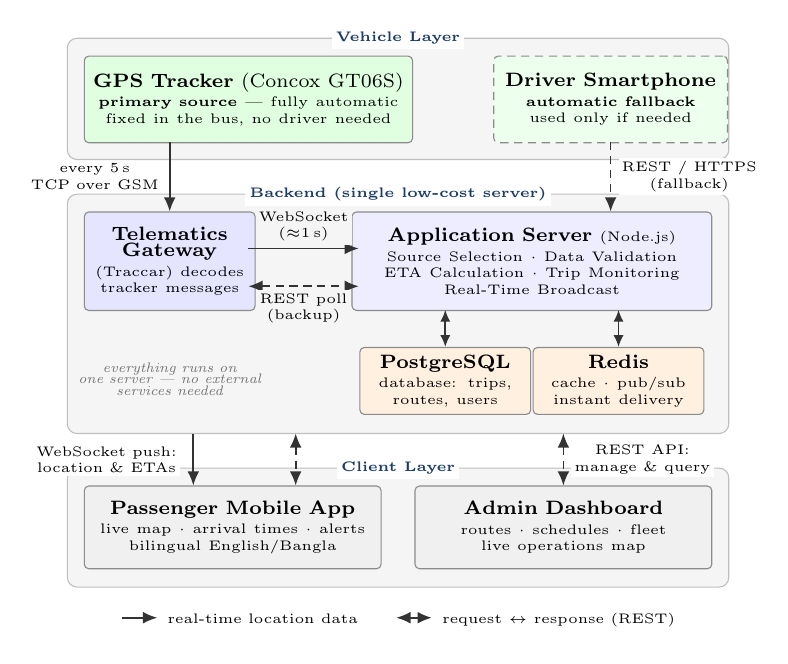
\begin{tikzpicture}[font=\scriptsize, x=1mm, y=1mm]
% ---------- layer panels (drawn first, boxes on top) ----------
\draw[panel] (-42, 2.2) rectangle ( 42,-13.2);
\draw[panel] (-42,-17.6) rectangle ( 42,-48.0);
\draw[panel] (-42,-52.4) rectangle ( 42,-67.5);
\node[zlab] at (0, 2.2)  {Vehicle Layer};
\node[zlab] at (0,-17.6) {Backend (single low-cost server)};
\node[zlab] at (0,-52.4) {Client Layer};
% ---------- vehicle layer ----------
\node[blk, fill=green!12, text width=40mm, minimum height=11mm, anchor=north] (gt) at (-19,0)
  {\textbf{GPS Tracker} (Concox GT06S)\\[-1pt]
   {\tiny \textbf{primary source} --- fully automatic}\\[-2pt]
   {\tiny fixed in the bus, no driver needed}};
\node[blk, fill=green!7, densely dashed, text width=28mm, minimum height=11mm, anchor=north]
  (ph) at (27,0)
  {\textbf{Driver Smartphone}\\[-1pt]
   {\tiny \textbf{automatic fallback}}\\[-2pt]
   {\tiny used only if needed}};
% ---------- backend layer ----------
\node[blk, fill=blue!10, text width=20mm, minimum height=12.5mm, anchor=north] (trac) at (-29,-19.8)
  {\textbf{Telematics}\\[-2pt]\textbf{Gateway}\\[-1pt]
   {\tiny (Traccar) decodes}\\[-2pt]{\tiny tracker messages}};
\node[blk, fill=blue!7, text width=44mm, minimum height=12.5mm, anchor=north] (app) at (17,-19.8)
  {\textbf{Application Server} {\tiny(Node.js)}\\[-1pt]
   {\tiny Source Selection $\cdot$ Data Validation}\\[-2pt]
   {\tiny ETA Calculation $\cdot$ Trip Monitoring}\\[-2pt]
   {\tiny Real-Time Broadcast}};
\node[blk, fill=orange!12, text width=20mm, minimum height=8.5mm, anchor=north] (pg) at (6,-37.0)
  {\textbf{PostgreSQL}\\[-1pt]{\tiny database: trips,}\\[-2pt]{\tiny routes, users}};
\node[blk, fill=orange!12, text width=20mm, minimum height=8.5mm, anchor=north] (rd) at (28,-37.0)
  {\textbf{Redis}\\[-1pt]{\tiny cache $\cdot$ pub/sub}\\[-2pt]{\tiny instant delivery}};
\node[font=\tiny\itshape, text=black!55, align=center] at (-29,-41.1)
  {everything runs on\\[-2pt]one server --- no external\\[-2pt]services needed};
% ---------- client layer ----------
\node[blk, fill=black!6, text width=36mm, minimum height=10.5mm, anchor=north] (pass) at (-21,-54.6)
  {\textbf{Passenger Mobile App}\\[-1pt]
   {\tiny live map $\cdot$ arrival times $\cdot$ alerts}\\[-2pt]
   {\tiny bilingual English/Bangla}};
\node[blk, fill=black!6, text width=36mm, minimum height=10.5mm, anchor=north] (adm) at (21,-54.6)
  {\textbf{Admin Dashboard}\\[-1pt]
   {\tiny routes $\cdot$ schedules $\cdot$ fleet}\\[-2pt]
   {\tiny live operations map}};
% ---------- connections (all verticals aligned to fixed x) ----------
\draw[arr]  (-29,-11) -- (-29,-19.8)
  node[lab, midway, anchor=east, xshift=-0.9mm] {every 5\,s\\TCP over GSM};
\draw[barr] ( 27,-11) -- ( 27,-19.8)
  node[lab, midway, anchor=west, xshift=0.9mm] {REST / HTTPS\\(fallback)};
\draw[arr]  (-19,-24.5) -- (-5,-24.5)
  node[lab, midway, anchor=south, yshift=0.4mm, fill=black!4] {WebSocket\\($\approx$1\,s)};
\draw[bbarr] (-19,-29.3) -- (-5,-29.3)
  node[lab, midway, anchor=north, yshift=-0.4mm, fill=black!4] {REST poll\\(backup)};
\draw[darr] ( 6,-32.3) -- ( 6,-37.0);
\draw[darr] (28,-32.3) -- (28,-37.0);
\draw[arr]  (-26,-48.0) -- (-26,-54.6)
  node[lab, midway, anchor=east, xshift=-1.6mm] {WebSocket push:\\location \& ETAs};
\draw[bbarr] (-13,-48.0) -- (-13,-54.6);
\draw[bbarr] ( 21,-48.0) -- ( 21,-54.6)
  node[lab, midway, anchor=west, xshift=0.9mm] {REST API:\\manage \& query};
% ---------- legend ----------
\node[anchor=north, font=\tiny] at (0,-69.4)
  {\tikz{\draw[arr] (0,0) -- (4.5mm,0);}\, real-time location data\qquad
   \tikz{\draw[bbarr] (0,0) -- (4.5mm,0);}\, request $\leftrightarrow$ response (REST)};
\end{tikzpicture}}%
\caption{UniBus Live system architecture. The GPS tracker is the primary,
fully automatic source; the driver's smartphone is only a fallback. All
backend components share one low-cost cloud server.}
\label{fig:architecture}
\end{figure}

\begin{figure}[H]
\centering
\resizebox{0.97\columnwidth}{!}{%
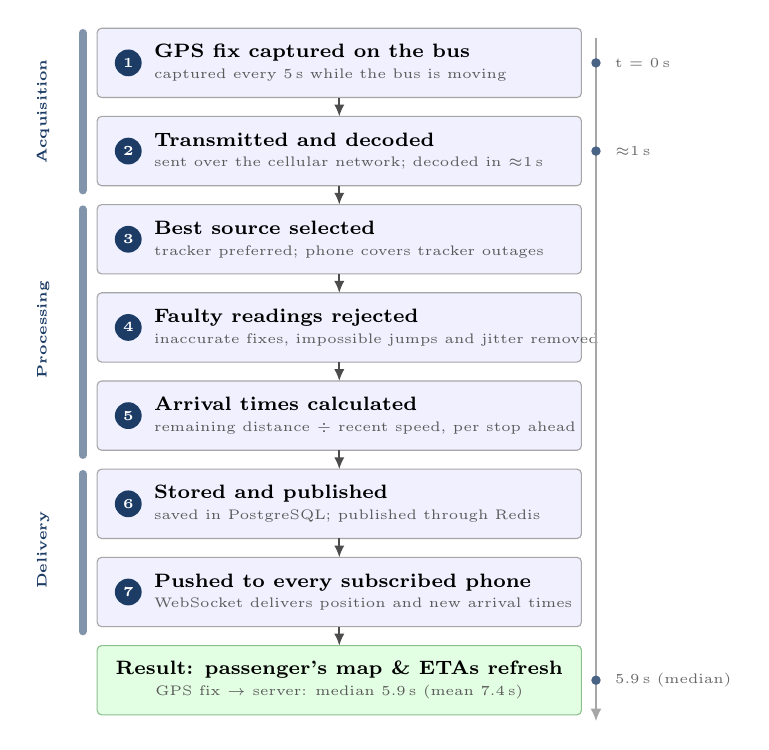
\begin{tikzpicture}[font=\scriptsize, x=1mm, y=1mm,
  stp/.style={draw=black!35, rounded corners=1.6pt, fill=blue!6, align=left,
              text width=58mm, minimum height=8.8mm, inner sep=2.2pt, anchor=north},
  sarr/.style={-{Latex[length=1.5mm,width=1.3mm]}, semithick, draw=black!70},
  phl/.style={font=\tiny\bfseries\scshape, text=acc, rotate=90, anchor=south}]
% ---- steps on a uniform grid: height 8.8, gap 2.4 ----
\foreach \y/\n/\t/\d in {
  0/1/{GPS fix captured on the bus}/{captured every 5\,s while the bus is moving},
  -11.2/2/{Transmitted and decoded}/{sent over the cellular network; decoded in $\approx$1\,s},
  -22.4/3/{Best source selected}/{tracker preferred; phone covers tracker outages},
  -33.6/4/{Faulty readings rejected}/{inaccurate fixes, impossible jumps and jitter removed},
  -44.8/5/{Arrival times calculated}/{remaining distance $\div$ recent speed, per stop ahead},
  -56.0/6/{Stored and published}/{saved in PostgreSQL; published through Redis},
  -67.2/7/{Pushed to every subscribed phone}/{WebSocket delivers position and new arrival times}}{
  \draw[draw=black!35, rounded corners=1.6pt, fill=blue!6]
    (-30.75,\y) rectangle (30.75,\y-8.8);
  \node[circle, fill=acc, text=white, inner sep=0.25mm, minimum size=3.4mm,
        font=\tiny\bfseries] at (-26.8,\y-4.4) {\n};
  \node[anchor=west, align=left, inner sep=0pt] at (-23.6,\y-4.4)
    {\textbf{\t}\\[-0.5pt]{\tiny\color{black!65} \d}};
}
\draw[draw=green!45!black!45, rounded corners=1.6pt, fill=green!11]
  (-30.75,-78.4) rectangle (30.75,-87.2);
\node[align=center] at (0,-82.8)
  {\textbf{Result: passenger's map \& ETAs refresh}\\[-0.5pt]
   {\tiny\color{black!65} GPS fix $\rightarrow$ server: median 5.9\,s (mean 7.4\,s)}};
% ---- identical arrows (2.4 mm each) ----
\foreach \y in {-8.8,-20.0,-31.2,-42.4,-53.6,-64.8,-76.0}{
  \draw[sarr] (0,\y) -- (0,\y-2.4);}
% ---- phase bars (left, uniform) ----
\foreach \ya/\yb/\nm in {0/-20.0/Acquisition, -22.4/-53.6/Processing, -56.0/-76.0/Delivery}{
  \draw[acc!55, line width=1mm, line cap=round] (-32.6,\ya-0.6) -- (-32.6,\yb-0.6);}
\node[phl] at (-35.6,-10.6) {Acquisition};
\node[phl] at (-35.6,-38.3) {Processing};
\node[phl] at (-35.6,-66.3) {Delivery};
% ---- timeline (right) ----
\draw[black!35, line width=0.6pt, -{Latex[length=1.6mm,width=1.4mm]}]
  (32.6,-1.2) -- (32.6,-88.0);
\foreach \y/\t in {-4.4/{t $=$ 0\,s}, -15.6/{$\approx$1\,s}, -82.8/{5.9\,s (median)}}{
  \fill[acc!80] (32.6,\y) circle (0.6mm);
  \node[font=\tiny, anchor=west, text=black!60] at (33.8,\y) {\t};}
\end{tikzpicture}}%
\caption{Real-time data flow: the life of one position report, from the
GPS fix on the bus to the passenger's screen, grouped into acquisition,
processing, and delivery phases. Steps 3--5 are detailed in
Sections~\ref{sec:impl-arbitration}--\ref{sec:impl-eta}.}
\label{fig:dataflow}
\end{figure}

\subsection{Application Server}
The server is implemented in TypeScript on Node.js using the Express
framework. Persistence is provided by PostgreSQL through the Prisma
object--relational mapper; the schema comprises 31 relational models
organised into six functional domains (Fig.~\ref{fig:datamodel}): identity and
authentication, fleet
and devices, routing and scheduling, trip and tracking, communications and
passenger, and audit and operations. An in-memory Redis instance serves two
roles: a short-lived cache for hot read paths and the publish/subscribe
back-plane for the WebSocket layer, letting the realtime tier scale
horizontally without losing fan-out consistency.
Realtime delivery uses Socket.IO, with each active trip represented as a
logical \emph{room}; a passenger tracking a trip joins that trip's room and
thereafter receives only its events, bounding per-client traffic to the
single vehicle being observed.

\begin{figure}[b]
\centering
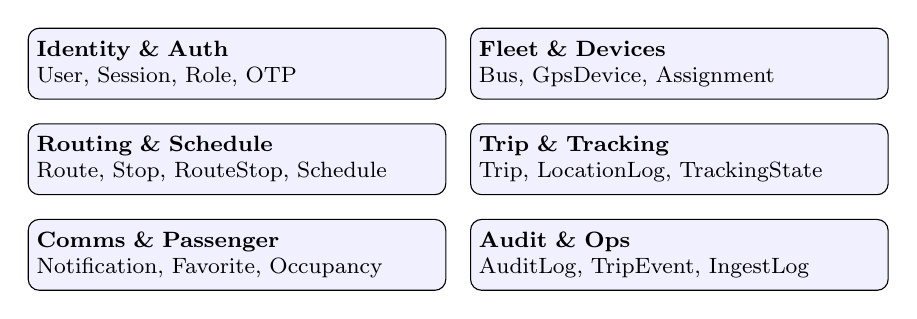
\begin{tikzpicture}[font=\footnotesize,
  dom/.style={draw, rounded corners, fill=blue!6, align=left,
              text width=0.42\columnwidth, inner sep=3pt, minimum height=9mm}]
  \node[dom] (a) {\textbf{Identity \& Auth}\\User, Session, Role, OTP};
  \node[dom, right=3mm of a] (b) {\textbf{Fleet \& Devices}\\Bus, GpsDevice, Assignment};
  \node[dom, below=3mm of a] (c) {\textbf{Routing \& Schedule}\\Route, Stop, RouteStop, Schedule};
  \node[dom, right=3mm of c] (d) {\textbf{Trip \& Tracking}\\Trip, LocationLog, TrackingState};
  \node[dom, below=3mm of c] (e) {\textbf{Comms \& Passenger}\\Notification, Favorite, Occupancy};
  \node[dom, right=3mm of e] (f) {\textbf{Audit \& Ops}\\AuditLog, TripEvent, IngestLog};
\end{tikzpicture}
\caption{The 31-model relational schema, grouped into six functional domains.}
\label{fig:datamodel}
\end{figure}

\subsection{GPS-Acquisition Layer}
Vehicle positions originate from two independent source types. The primary
source is a fixed, vehicle-grade Concox~GT06S GPS/GSM tracker hard-wired to
the bus, reporting to a self-hosted Traccar telematics server. An optional
secondary source is the driver's smartphone, which can publish location
through an authenticated REST endpoint when no hardware fix is available;
normal operation uses the tracker alone and requires no driver device,
action, or connectivity. The
application server ingests Traccar data through two complementary paths: a
session-cookie WebSocket subscription that \emph{pushes} each new fix within
about a second of Traccar receiving it, backed by an 8\,s REST polling job as a
fallback when the socket is unavailable. It then reconciles the two source
types through a source-arbitration component
(Section~\ref{sec:impl-arbitration}). Both Traccar and the application
server are self-hosted on a single low-cost virtual private server, keeping
recurring infrastructure cost within a student-project budget.

\subsection{Client Applications}
The passenger application is built with React Native and Expo, rendering live
vehicle and route geometry on a map. It uses a foreground location service
for continued tracking while backgrounded and push notifications for alerts,
and its interface is fully bilingual (English and Bangla); representative
passenger screens are shown in Fig.~\ref{fig:screens}. The administration
console is a server-rendered React (Next.js) application integrating the
Google Maps JavaScript API for the live operations map and the route-builder
tool; it also manages buses, GPS devices, schedules, and user roles through
the same REST API.

% =====================================================================
\section{Implementation}
\label{sec:implementation}

\subsection{Location Ingestion and Multi-Source Arbitration}
\label{sec:impl-arbitration}
Each inbound fix---polled from Traccar, pushed over its WebSocket, or posted
by a driver device---is recorded with both its device-reported timestamp and
its server-receipt timestamp, and tagged with its source. For every bus the
server maintains one \emph{source-tracking state} per active source and a
single \emph{canonical tracking state} representing the position passengers
see. When a hardware tracker and a driver phone are both live, an arbitration
routine selects the canonical source by health score and a configurable
priority rank, preferring a healthy hardware tracker but transparently
falling back to the phone if the tracker goes silent. Because arbitration
operates per fix, a bus can hand over between sources mid-trip without any
passenger-visible artefact: the canonical marker simply continues from the
freshest healthy source. Every accepted fix is also appended to a per-trip
location log, preserving the complete trajectory for later analysis.

\begin{figure*}[t]
\centering
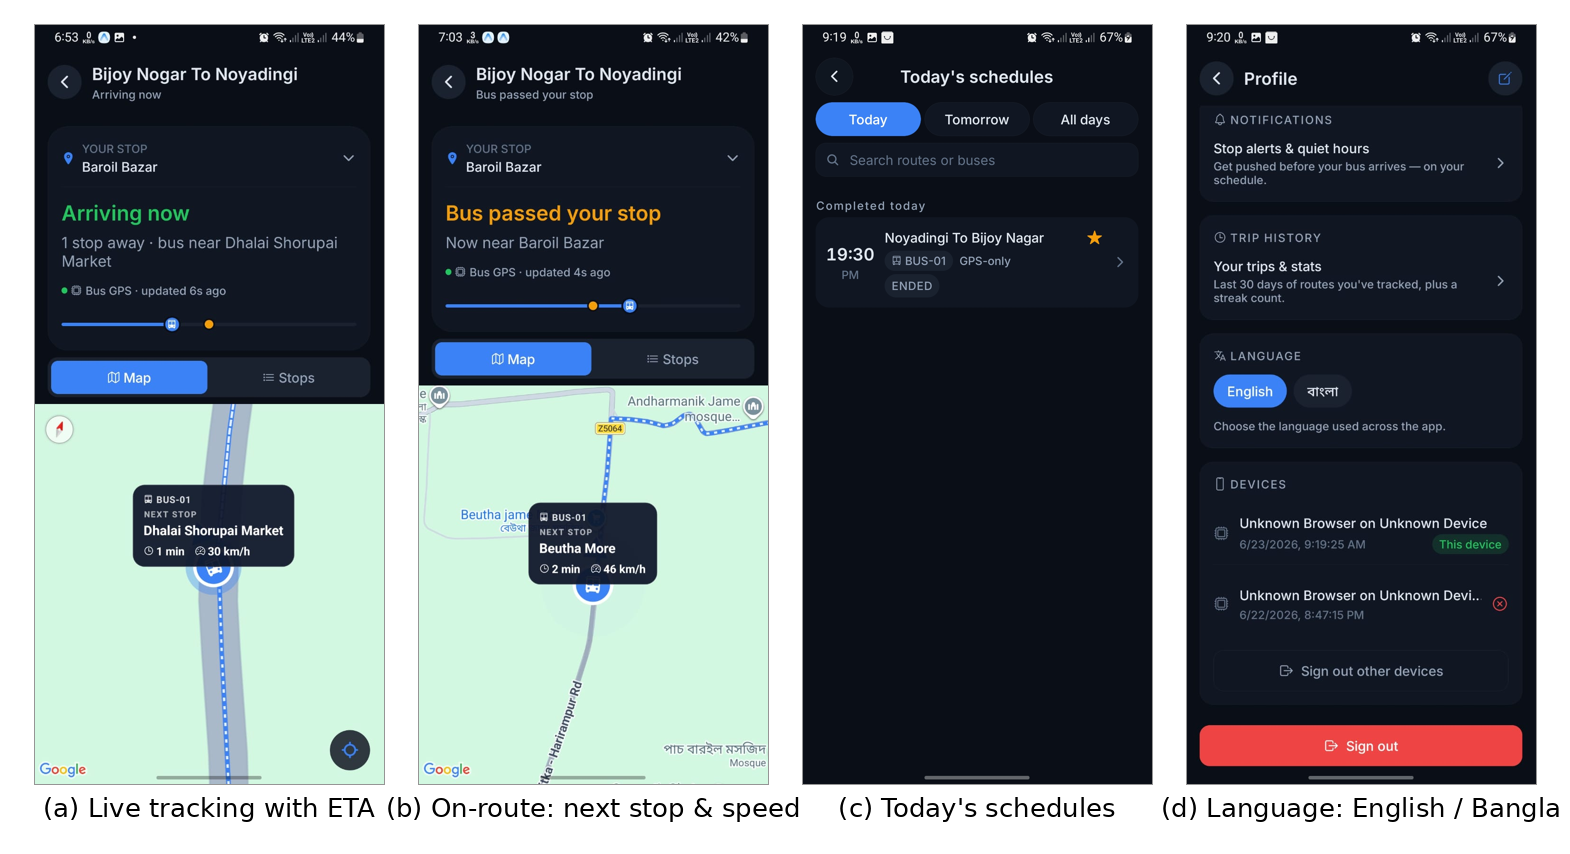
\includegraphics[width=0.85\textwidth]{screens.png}
\caption{The bilingual passenger application. (a) live tracking of a moving bus
with the next-stop ETA; (b) on-route status showing the next stop and current
speed; (c) today's schedules; (d) the in-app English/Bangla language toggle.
Place names render in both scripts.}
\label{fig:screens}
\end{figure*}

\subsection{Location-Quality Filtering}
\label{sec:impl-filter}
A filtering pipeline gates every fix before it can move the canonical
position. The principal, operator-configurable rules are: (i)~an accuracy
gate that soft-rejects fixes worse than 120\,m and hard-rejects those worse
than 250\,m; (ii)~a teleport guard that rejects implied inter-fix speeds
above 120\,km/h; (iii)~a minimum-movement threshold of 4\,m below which the
bus is treated as stationary, suppressing GPS jitter; and (iv)~a
freeze/release hysteresis that holds the marker still under poor accuracy and
resumes motion only on a confident displacement. A short-window rolling
average of accepted speeds is maintained per trip and feeds the ETA
estimator. The thresholds are deliberately conservative: 120\,km/h exceeds
any plausible speed on the pilot routes, and the 4\,m floor sits above the
tracker's typical urban scatter, so legitimate motion is never suppressed.

\subsection{Arrival-Time Estimation}
\label{sec:impl-eta}
ETAs are computed geometrically against the ordered list of route stops. The
route is first reduced to a cumulative along-path distance array. The current
fix is projected onto the nearest route segment using a planar (local
equirectangular) projection, yielding the bus's progress distance and
cross-track offset; this makes the estimate robust to lateral GPS error and
to the bus being slightly off the idealised polyline. The remaining distance
to each upcoming stop is the difference between that stop's cumulative
distance and the bus's progress, divided by an effective speed---the per-trip
rolling-average speed when reliable ($\geq 5$\,km/h), otherwise a configurable
default of 20\,km/h---to yield a per-stop ETA, so a rider receives an estimate
for their own chosen stop rather than only the next one. Each estimate carries
a \textsc{high}/\textsc{medium}/\textsc{low} confidence label derived from the
speed-signal quality. A stop is marked reached when the bus enters an 80\,m
arrival radius, triggering a stop-arrival event and, for subscribed riders, a
push notification. The procedure is summarised in Algorithm~\ref{alg:eta}.

\begin{algorithm}[!t]
\fontsize{9.0}{11.0}\selectfont
\caption{Estimating the ETA to every upcoming stop}
\label{alg:eta}
\begin{algorithmic}[1]
\Require current bus GPS fix; ordered route stops; recent average speed
\Ensure an ETA and a confidence label for each stop ahead
\State Compute each stop's distance from the route start (cumulative)
\State Project the bus fix onto the nearest route segment to find how far
  along the route it has travelled (its \emph{progress})
\If{recent average speed $\geq 5$\,km/h}
  \State $speed \gets$ recent average speed
\Else
  \State $speed \gets 20$\,km/h \Comment{fallback default}
\EndIf
\ForAll{stops ahead of the bus}
  \State $remaining \gets (\text{stop's distance}) - (\text{progress})$
  \State $\text{ETA} \gets remaining / speed$
\EndFor
\State Assign a confidence (High/Medium/Low) from the speed quality
\If{the nearest stop is within 80\,m}
  \State mark it reached and notify subscribed riders
\EndIf
\State \Return the ETA and confidence for every stop ahead
\end{algorithmic}
\end{algorithm}

\subsection{Trip Lifecycle and Pre-Trip Awareness}
\label{sec:impl-lifecycle}
A trip transitions through
\textsc{planned}~$\rightarrow$~\textsc{pre\_trip}~$\rightarrow$~%
\textsc{running}~$\rightarrow$~\textsc{ended}. A scheduled job opens a
pre-trip window before the scheduled departure, during which the rider sees
the bus's pre-departure state (parked, approaching origin, or arrived at
origin) rather than a blank map; the vehicle auto-promotes to \textsc{running}
on dwelling inside the origin geofence. A staleness job runs every 30\,s and
flags trips whose last fix has aged beyond a threshold, so a frozen marker is
shown as stale rather than live.

\subsection{Realtime Delivery and Offline Behaviour}
\label{sec:impl-realtime}
Accepted canonical updates and recomputed ETAs are published to the relevant
per-trip room and, through the Redis adapter, to peer server processes
holding subscribers for that trip; authentication is enforced on socket
connection and room join. The client retains the most recent state so a
transient disconnection degrades to a ``last known'' view with an explicit
staleness indicator, and the passenger app renders the bus at the route
origin during the pre-trip phase so the live map is never blank while a rider
waits.

\subsection{Device-Side Reporting Configuration}
\label{sec:impl-device}
The server-side throttling described in Section~\ref{sec:eval-discussion}
reduces redundant \emph{ingestion}, but the tracker still transmitted a fix
every few seconds while parked, draining the bus battery and consuming
cellular data at the device itself. Because the Concox~GT06S is configured
over SMS, we set an asymmetric reporting cadence directly on the unit:
\texttt{TIMER,5,300\#} makes the tracker report every 5\,s while moving but
only every 300\,s while static; \texttt{PARAM\#} reads back the active
configuration and \texttt{STATUS\#} the battery and GSM/GPS state, each
acknowledged by return SMS. This cadence is the transmission-layer
counterpart to the server-side gate (Table~\ref{tab:efficiency}). We
verified the change from two independent vantage points---the per-position
timestamps in the Traccar report view and the server's own ingest
log---confirming parked-state fixes spaced by minutes rather than seconds,
while a live test drive still produced dense five-second fixes. A
low-frequency heartbeat keeps the device visible online between reports;
wiring the ignition (ACC) line for engine-state-triggered sleep is
identified as future work.

% =====================================================================
\section{Evaluation}
\label{sec:evaluation}

\subsection{Deployment and Dataset}
UniBus Live was evaluated in a seven-week pilot (6~May--23~June~2026) on an
operational university fleet. Table~\ref{tab:dataset} summarises the dataset.
The deployment covered 9 routes and 3 buses (one equipped with a fixed
hardware tracker), served 38 registered passenger accounts, and recorded 71
completed trips during which 46{,}548 raw GPS reports were ingested. Of these,
only 864 were retained as in-trip fixes; the remaining ${\sim}98\%$ were
redundant reports transmitted while buses were parked---an inefficiency we
quantify and address in Section~\ref{sec:evaluation} (Table~\ref{tab:efficiency}).
We report results from operational data; figures are representative of a small
pilot rather than a city-scale deployment.

\begin{table}[H]
\caption{Pilot Deployment Summary}
\label{tab:dataset}
\centering
\begin{tabular}{lr}
\toprule
\textbf{Quantity} & \textbf{Value} \\
\midrule
Deployment span            & 7 weeks \\
Routes                     & 9 \\
Buses                      & 3 \\
Registered passengers      & 38 \\
Completed trips            & 71 \\
Raw GPS reports ingested   & 46{,}548 \\
In-trip fixes retained     & 864 \\
Mean GPS fixes per trip    & 37.6 \\
\bottomrule
\end{tabular}
\end{table}

\subsection{Methodology}
All metrics are computed from the production database. Position-acquisition
latency is the difference between each fix's device timestamp and its
server-receipt timestamp. Source-fallback usage is taken from the canonical
source selected per trip. ETA accuracy is measured by logging every predicted
arrival instant and later comparing it against the corresponding recorded stop
arrival; we report the mean absolute error.

\subsection{Results}

\subsubsection{Position-acquisition latency}
Across 46{,}286 fixes, the median latency from device fix to server receipt
was 5.9\,s (mean 7.4\,s; 90th percentile 9.9\,s; 95th percentile 11.1\,s).
This is bounded primarily by the 8\,s Traccar polling interval rather than by
network transport. A further median 1.2\,s elapsed before a fix was persisted.

\subsubsection{Source resilience}
The dual-source design was exercised in practice rather than remaining a
theoretical safeguard: 64\% of trips (45 of 70 with a recorded source) were
tracked via the fixed hardware tracker and 36\% (25) via the smartphone
fallback. This confirms that the fallback path carried a substantial share of
real trips, sustaining coverage when hardware fixes were
unavailable---largely reflecting trips by the two buses not yet fitted with
trackers. The design remains hardware-first: the tracker operates with no
driver involvement, and as trackers are fitted fleet-wide the smartphone
path reduces to a rarely needed, optional safety net.

\subsubsection{ETA estimation}
The geometric estimator produces a per-stop arrival prediction on every
accepted fix, each carrying a \textsc{high}/\textsc{medium}/\textsc{low}
confidence label. To support quantitative accuracy assessment, the system
logs every predicted arrival instant so that the mean absolute error
against recorded stop arrivals can be measured as operational data
accumulates over continued deployment.

\subsubsection{Passenger engagement}
Of 45 arrival/service notifications delivered during the pilot, 36 (80\%) were
read, indicating that the passenger-facing alerts were attended to.

\subsection{Limitations}
The pilot is small in scale and duration, a subset of trips were operational
tests, and one bus carried the hardware tracker; results should therefore be
read as a feasibility demonstration. The hardware tracker does not report a
per-fix accuracy value, so quality filtering is evaluated at the trip level
rather than per fix. Schedule-adherence analysis was limited by incomplete
timetable association during the pilot.

\subsection{Discussion: Toward Adaptive Location Reporting}
\label{sec:eval-discussion}
A notable observation from the pilot is that of the 46{,}548 raw device
reports, only 864 were retained as in-trip fixes: the fixed-interval tracker
transmitted continuously even while buses were parked, so roughly 98\% of
reports fell outside any active trip. For a \emph{scheduled} fleet this wastes
cellular data and, for a tracker wired to the vehicle battery, stored charge.
A more efficient design couples reporting to vehicle state and the timetable:
ignition- and motion-triggered reporting (dense while moving, a sparse
heartbeat while parked), distance-based thresholds, and server-side gating of
heavy processing to scheduled trip windows---which the system's existing
pre-trip window already approximates. Motivated by this observation, we implemented both halves of this strategy:
server-side trip-aware throttling that restricts full-rate polling to buses
in an active trip or pre-trip window, dropping parked buses to a slow
heartbeat while leaving on-trip tracking and the WebSocket push path
unaffected; and device-side reconfiguration to 5\,s moving / 300\,s parked
(versus a uniform 5\,s previously; Section~\ref{sec:impl-device}),
curtailing transmissions, battery drain, and cellular-data use at the
source. Finer-grained sleep and distance-based reporting are left as future
work. As summarised in
Table~\ref{tab:efficiency}, these changes cut parked-state reporting by roughly
$60\times$ at the device and idle polling by $7.5\times$ at the server, directly
targeting the 98\% of reports that the pilot showed were redundant. After the optimization the server ingests
essentially only the dense fixes produced during active trips plus a sparse
five-minute parked heartbeat per bus, rather than the previous continuous
five-second stream.

\begin{table}[H]
\caption{Idle-Reporting Efficiency Optimization}
\label{tab:efficiency}
\centering
\begin{tabular}{llrr}
\toprule
\textbf{Layer} & \textbf{Parameter} & \textbf{Before} & \textbf{After} \\
\midrule
Device (GT06S) & Parked report interval & 5\,s & 300\,s \\
Server         & Idle poll interval     & 8\,s & 60\,s \\
\bottomrule
\end{tabular}
\end{table}

% =====================================================================
\section{Conclusion and Future Work}
\label{sec:conclusion}
We presented UniBus Live, a deployed real-time university bus tracking system
distinguished by resilient dual-source GPS acquisition, a lightweight
geometric ETA estimator, and a bilingual, edge-condition-aware passenger
experience. A seven-week pilot on a real fleet demonstrated feasibility: the
system ingested 46{,}548 GPS reports across 71 trips with a median acquisition
latency of 5.9\,s, and its optional smartphone-fallback path carried 36\% of trips (largely
buses awaiting tracker installation), validating graceful degradation while
normal operation requires no driver device. The pilot also exposed that roughly 98\% of
device reports were redundant idle-state transmissions; we eliminated this
waste through a two-sided optimization---server-side trip-aware throttling and
device-side interval reconfiguration---cutting idle-period reporting by up to
$60\times$ without affecting on-trip tracking. Future work includes
learning-based ETA prediction using the accumulating trajectory history, full
timetable integration for schedule-adherence analytics, crowd-sourced
occupancy at larger scale, and a wider, longer deployment with a formal
passenger usability study.

% =====================================================================
\section*{Acknowledgment}
The authors thank Mahbubur Rahman Chowdhury for supervision, and the
Department of Computer Science and Engineering, NPI University of Bangladesh.

% =====================================================================
\begin{thebibliography}{00}
\bibitem{sharif2018}
S.~A. Sharif, M.~S.~A. Suhaimi, N.~N. Jamal, I.~K. Riadz, I.~F. Amran, and
D.~N.~A. Jawawi, ``Real-time campus university bus tracking mobile
application,'' in \textit{Proc. 7th ICT Int. Student Project Conf.
(ICT-ISPC)}, 2018.
\bibitem{premkumar2020}
K.~Premkumar, K.~Pavithra, J.~Presiela, D.~Priyadarshini, and P.~Priyanga,
``College bus tracking and notification system,'' in \textit{Proc. Int. Conf.
System, Computation, Automation and Networking (ICSCAN)}, 2020.
\bibitem{zhou2012}
P.~Zhou, Y.~Zheng, Z.~Li, M.~Li, and G.~Shen, ``How long to wait? Predicting
bus arrival time with mobile phone based participatory sensing,'' in
\textit{Proc. 10th ACM Int. Conf. Mobile Systems, Applications, and Services
(MobiSys)}, 2012.
\bibitem{wepulanon2018}
P.~Wepulanon, A.~Sumalee, and W.~H.~K. Lam, ``A real-time bus arrival time
information system using crowdsourced smartphone data: a novel framework and
simulation experiments,'' \textit{Transportmetrica B: Transport Dynamics},
vol.~6, no.~1, 2018.
\bibitem{reich2019}
T.~Reich, M.~Budka, D.~Robbins, and D.~Hulbert, ``Survey of ETA prediction
methods in public transport networks,'' \textit{arXiv preprint
arXiv:1904.05037}, 2019.
\bibitem{singh2022}
N.~Singh and K.~Kumar, ``A review of bus arrival time prediction using
artificial intelligence,'' \textit{WIREs Data Mining and Knowledge Discovery},
vol.~12, no.~4, p.~e1457, 2022.
\bibitem{ye2020}
L.~Ye and P.~Thiengburanathum, ``A real-time bus arrival time prediction
system based on Spark framework and machine learning approaches: a case study
in Chiang Mai,'' in \textit{Proc. Joint Int. Conf. Digital Arts, Media and
Technology (ECTI DAMT \& NCON)}, 2020.
\bibitem{rashvand2023}
N.~Rashvand, S.~S. Hosseini, M.~Azarbayjani, and H.~Tabkhi, ``Real-time bus
arrival prediction: a deep learning approach for enhanced urban mobility,''
\textit{arXiv preprint arXiv:2303.15495}, 2023.
\bibitem{rashvand2024}
N.~Rashvand, M.~Azarbayjani, S.~S. Hosseini, and H.~Tabkhi, ``Real-time bus
departure prediction using neural networks for smart IoT public bus
transit,'' \textit{IoT}, vol.~5, no.~4, pp.~650--665, 2024.
\bibitem{jeong2024}
S.~Jeong, C.~Oh, and J.~Jeong, ``BAT-Transformer: prediction of bus arrival
time with transformer encoder for smart public transportation system,''
\textit{Applied Sciences}, vol.~14, no.~20, art.~9488, 2024.
\bibitem{barnes2020}
R.~Barnes, S.~Buthpitiya, J.~Cook, A.~Fabrikant, A.~Tomkins, and F.~Xu,
``BusTr: Predicting bus travel times from real-time traffic,'' in
\textit{Proc. 26th ACM SIGKDD Int. Conf. Knowledge Discovery \& Data Mining
(KDD)}, 2020, pp.~3243--3251.
\bibitem{newson2009}
P.~Newson and J.~Krumm, ``Hidden Markov map matching through noise and
sparseness,'' in \textit{Proc. 17th ACM SIGSPATIAL Int. Conf. Advances in
Geographic Information Systems}, 2009, pp.~336--343.
\bibitem{traccar}
``Traccar: Open source GPS tracking platform.'' \url{https://www.traccar.org/}
\end{thebibliography}

\end{document}
